
%(BEGIN_QUESTION)
% Copyright 2011, Tony R. Kuphaldt, released under the Creative Commons Attribution License (v 1.0)
% This means you may do almost anything with this work of mine, so long as you give me proper credit

A ``smart'' (digital) DP flow transmitter configured for square-root characterization is removed from service and taken to a calibration bench for testing.  A technician connects a precision pressure gauge and air source to the transmitter's high port while monitoring the 4-20 mA output signal using a DMM:

$$\includegraphics[width=15.5cm]{i03473x01.eps}$$

Determine what {\bf PV} and {\bf AO} values will be displayed on the HART communicator display if the calibration error lies entirely in the sensor (i.e. the transmitter requires a sensor trim) versus if it lies entirely in the digital-analog converter (i.e. the transmitter requires an output trim).

% No blank lines allowed between lines of an \halign structure!
% I use comments (%) instead, so that TeX doesn't choke.

$$\vbox{\offinterlineskip
\halign{\strut
\vrule \quad\hfil # \ \hfil & 
\vrule \quad\hfil # \ \hfil & 
\vrule \quad\hfil # \ \hfil \vrule \cr
\noalign{\hrule}
%
% First row
{\bf Parameter} & {\bf If sensor trim error} & {\bf If output trim error} \cr
%
\noalign{\hrule}
%
% Another row
PV &  &  \cr
%
\noalign{\hrule}
%
% Another row
AO &  &  \cr
%
\noalign{\hrule}
} % End of \halign 
}$$ % End of \vbox

\vfil 

\underbar{file i03473}
\eject
%(END_QUESTION)





%(BEGIN_ANSWER)

This is a graded question -- no answers or hints given!

%(END_ANSWER)





%(BEGIN_NOTES)

% No blank lines allowed between lines of an \halign structure!
% I use comments (%) instead, so that TeX doesn't choke.

An important principle to bear in mind here is that the digital microprocessor inside the smart transmitter never makes arithmetic errors -- it {\it always} calculates the proper AO value for any given PV value.  Therefore, we should {\it always} expect the PV and AO figures displayed by the HART communicator to correspond perfectly with one another.

What will happen if there is a sensor trim error is that the transmitter will not ``see'' the real applied pressure: for any pressure applied to the sensor, the transmitter will register a PV value that is something different, and from there it will calculate what it thinks should be the correct milliamp output signal value.

If, however, there is an output (digital-to-analog converter) error, the transmitter will calculate the correct output signal value (AO) but this will not become the real milliamp current value output by the transmitter.

In summary, sensor trim errors cause the real input pressure to deviate from the PV value ``seen'' by the transmitter, while output trim errors cause the real current signal to deviate from the AO value calculated by the transmitter.  In no case will a trim error cause the PV and AO values to not correspond, because they are digitally calculated by the microprocessor which always performs perfect arithmetic.

\vskip 10pt

For more help understanding these concepts, refer to this simplified block diagram of a ``smart'' pressure transmitter with analog (4-20 mA) output:

$$\includegraphics[width=15.5cm]{i03473x02.eps}$$

\vskip 10pt

\filbreak

If the calibration error lies within the transmitter's sensor, then the analog output (AO) will read the same as the DMM and the process variable (PV) will deviate from the digital pressure gauge.  To predict the transmitter's PV and AO values, we set AO equal to the meter's indication (13.93 mA) and calculate what amount of sensed pressure would correspond to that amount of signal current.

\vskip 10pt

If the calibration error lies within the transmitter's output (DAC), then the analog output (AO) will deviate from the DMM and the process variable (PV) will read the same as the digital pressure gauge.  To predict the transmitter's PV and AO values, we set the PV equal to the pressure gauge's indication (37.80 "WC) and calculate what amount of output current would correspond to that amount of input pressure.

$$\vbox{\offinterlineskip
\halign{\strut
\vrule \quad\hfil # \ \hfil & 
\vrule \quad\hfil # \ \hfil & 
\vrule \quad\hfil # \ \hfil \vrule \cr
\noalign{\hrule}
%
% First row
{\bf Parameter} & {\bf If sensor trim error} & {\bf If output trim error} \cr
%
\noalign{\hrule}
%
% Another row
PV & 38.52 inH2O & 37.80 inH2O \cr
%
\noalign{\hrule}
%
% Another row
AO & 13.93 mA & 13.84 mA \cr
%
\noalign{\hrule}
} % End of \halign 
}$$ % End of \vbox


%INDEX% Calibration, smart transmitter: digital trim
%INDEX% Fieldbus, HART: communicator variables
%INDEX% Measurement, flow: square root characterized pressure transmitter

%(END_NOTES)

